\documentclass[fullpage,a4paper]{article}

\usepackage{amsmath}
\usepackage{amssymb}
\usepackage{amsthm}
\usepackage{bm}
\usepackage{authblk}
\usepackage{graphicx}
\usepackage{csquotes}
\usepackage{todonotes}
\usepackage{listings}
\usepackage{url}

\renewcommand{\v}[1]{\bm{#1}}
\newcommand{\vx}{\v{x}}
\newcommand{\vt}{\v{\theta}}
\newcommand{\vb}{\v{\beta}}
\newcommand{\vm}{\v{m}}
\newcommand{\R}{\mathbb{R}}
\newcommand{\E}{\mathbb{E}}
\newcommand{\Var}{\mathbb{V}ar}
\renewcommand{\P}{\mathbb{P}}
\newcommand{\Q}{\mathbb{Q}}
\newcommand{\D}{\mathcal{D}}

\newcommand{\eq}[1]{Equation~(\ref{eq:#1})}
\newcommand{\fig}[1]{Figure~\ref{fig:#1}}
\newcommand{\hyp}[1]{Assumption~\ref{hyp:#1}}

\newtheorem{definition}{Definition}
\newtheorem{hypothesis}{Assumption}
\newtheorem{theorem}{Theorem}

\newcommand{\beginsupplement}{%
  \setcounter{table}{0}
  \renewcommand{\thetable}{S\arabic{table}}%
  \setcounter{figure}{0}
  \renewcommand{\thefigure}{S\arabic{figure}}%
}

\title{A visual explanation of country specific differences in
  Covid-19 data.}
\author{Nils Bertschinger}

\begin{document}

\maketitle%%

\begin{abstract}
  This report provides a visual examination of Covid-19 case and death
  data. In particular, it shows that country specific differences can
  too a large extend be explained by two easily interpreted
  parameters. Namely, the delay between reported cases and deaths and
  the fraction of cases observed. Furthermore, this allows to lower
  bound the actual total number of people already infected.
\end{abstract}

\section{Introduction}

The unfolding COVID-19 pandemic requires timely and finessed
actions. Policy makers around the globe are hard pressed to balance
mitigation measures such as social distancing and economic
interests. While initial studies \cite{imperial1} predicted millions
of potential deaths never findings hint at a much more modest outcome
\cite{Lourenco2020.03.24.20042291,imperial2}. Especially the case
fatality rate (CFR) and the number of unobserved infections are
crucial to judge the state of the pandemic as well as the
effectiveness of its mitigation. Yet, there estimates are plaqued with
high uncertainties as exemplified in the quick revisions even from the
same institution \cite{imperial1,imperial2}

Most studies are based on elaborate epidemic modeling either using
stochastic or deterministic transmission dynamics. Especially, the
susceptible-infected-recovered (SIR) model \cite{Newman} forms a
basic building block and has been extended in several directions in
order to understand the dynamics of the ongoing Covid-19 pandemic
\cite{arxiv:2002.07572,arxiv:2004.01105,10.1126/science.abb3221,https://www.medrxiv.org/content/10.1101/2020.02.27.20028639v2}.
In this context, it has not only been compared with more
phenomenological growth models
\cite{https://doi.org/10.1101/2020.03.12.20034595}, e.g. logistic
growth, but also been used to quantify the effectiveness of quarantine
and social distancing \cite{arxiv:2002.07572,arxiv:2004.01105}.
E.g. social distancing, can be easily included by replacing the
infection rate parameter with a function allowing it to change over
time. \cite{arxiv:2004.01105} assumes one or several (soft) step
functions where the infection rate drops in response to different
measures after these had been implemented.

Unfortunately, building and fitting sufficiently complex models is not
without substantial model risk. While models might be well capable of
replicating observed data, predictions -- especially during the course
of an exponentially growing epidemic -- are often sensitive to
seemingly small details of model assumptions. They could even be
non-identified in important ways. Here, I show that this is indeed the
case for SIR type models with respect to the CFR and fraction of
observed infections.

Instead, a direct visual exploration of the data leads to valuable
insights. In particular, I show that much of the variability relating
reported case and death counts can be explained by two easily
interpreted parameters. Furthermore, building on three simple
assumptions this allows to lower bound the number of actual
infections, including observed and unobserved cases. In turn,
confirming recent estimates without complex and questionable modeling
choices.

\section{Data exploration}

Covid-19 data are published by several sources, most notably the John
Hopkins university and the European Center for Decease Prevention and
Control (ECDC). Here, data from ECDC as available from
\url{https://opendata.ecdc.europa.eu/covid19/casedistribution/csv} are
used.

\begin{figure}
  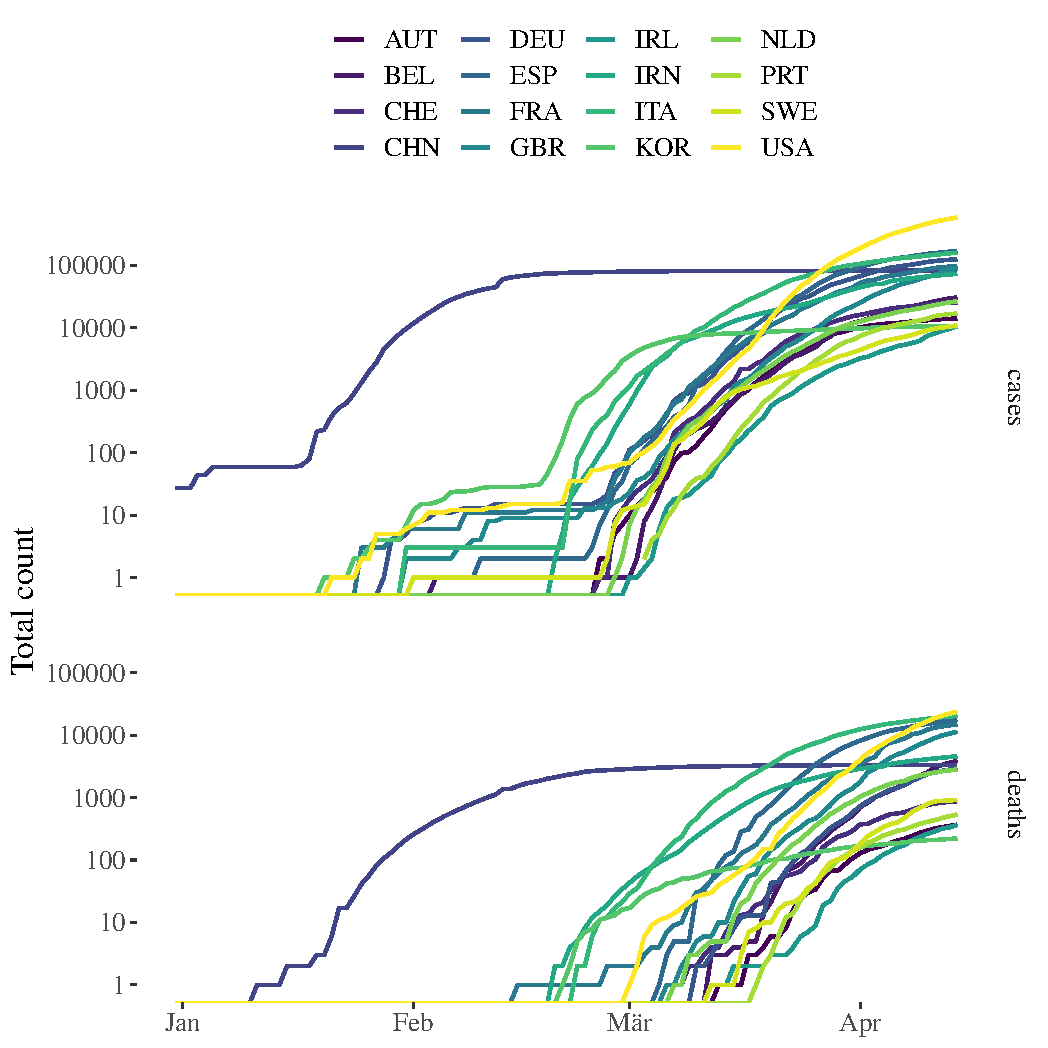
\includegraphics[width=0.495\textwidth]{../figs/ecdc_raw_absolute.pdf}
  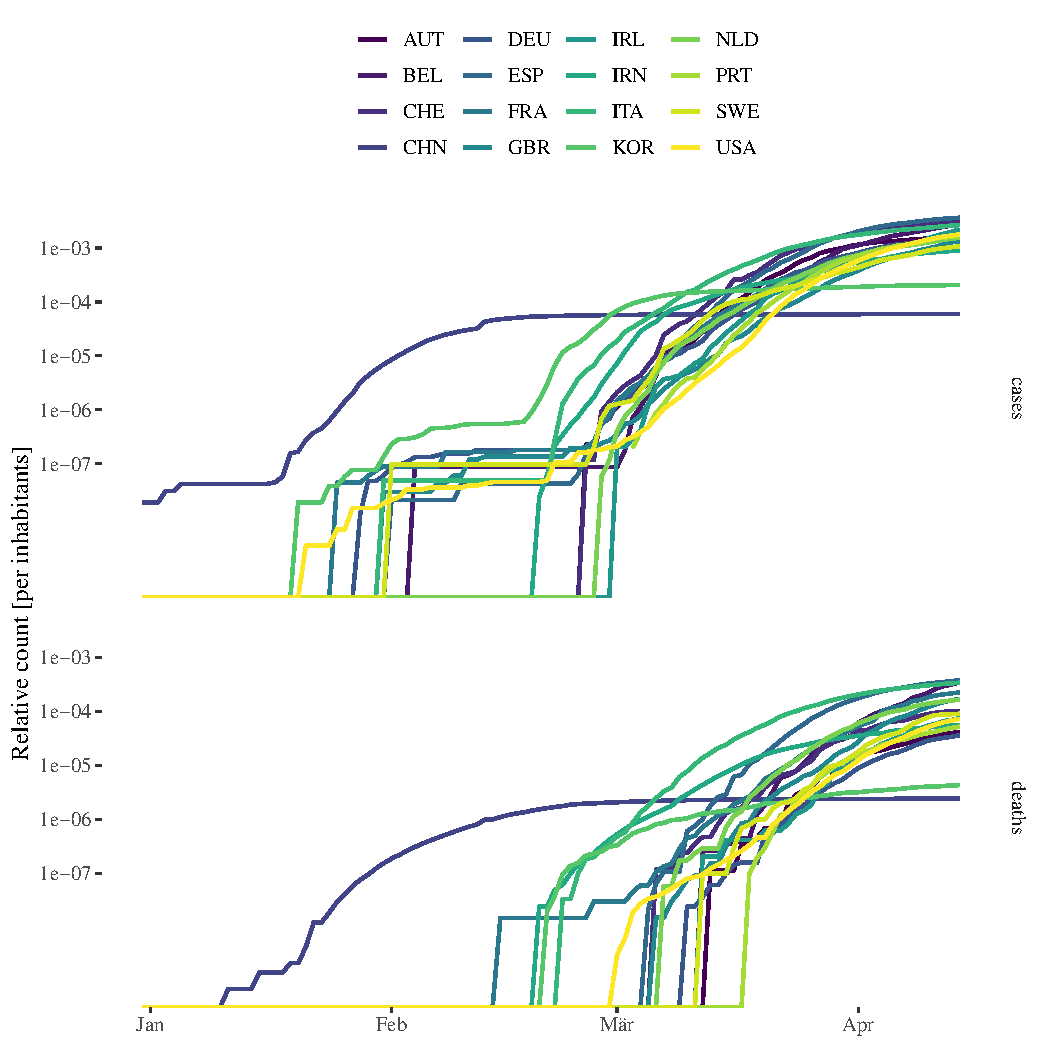
\includegraphics[width=0.495\textwidth]{../figs/ecdc_raw_relative.pdf}
  \caption{\label{fig:raw_data} Case and death counts of selected
    countries. Both in absolute (left) and relative (right), i.e. per
    inhabitants, terms.}
\end{figure}
\fig{raw_data} shows the total cumulative case and death counts of
selected countries. These countries are among the eight most effected
countries in terms of absolute and relative deaths\footnote{In
  addition, South Korea is included as its numbers are commonly
  considered of high quality.}. In the following, I will focus on
relative counts as these are arguably more meaningful when comparing
different countries -- which could differ widely in terms of
population size.

\begin{hypothesis}
  \label{hyp:count}
  Death counts are more reliable than case counts.
\end{hypothesis}

By \hyp{count} analysis will start from relative cumulative death
counts $d_t$ in the following\footnote{Similarly, relative cumulative
  case counts are denoted as $c_t$}. Furthermore, in order to
facilitate country comparisons, dates are shifted relative to the
first day that relative death counts exceed a threshold $\theta$ of
$1, 2, 4$ or $8$ deaths per million inhabitants respectively, i.e. $t
= 0$ is defined such that $d_t \geq \theta$ for $t \geq 0$ and $d_t <
\theta$ for $t < 0$. \fig{aligned_data} shows the resulting time
course of relative case and death counts. Aligning dates in this
fashion shows that several countries exhibit similar time courses,
e.g. Belgium and Spain or China and South Korea. Yet, there are
unexplained country specific differences and the data collapse is not
as complete as often observed in physical systems exhibiting scaling
laws \cite{stanley99}.
\begin{figure}
  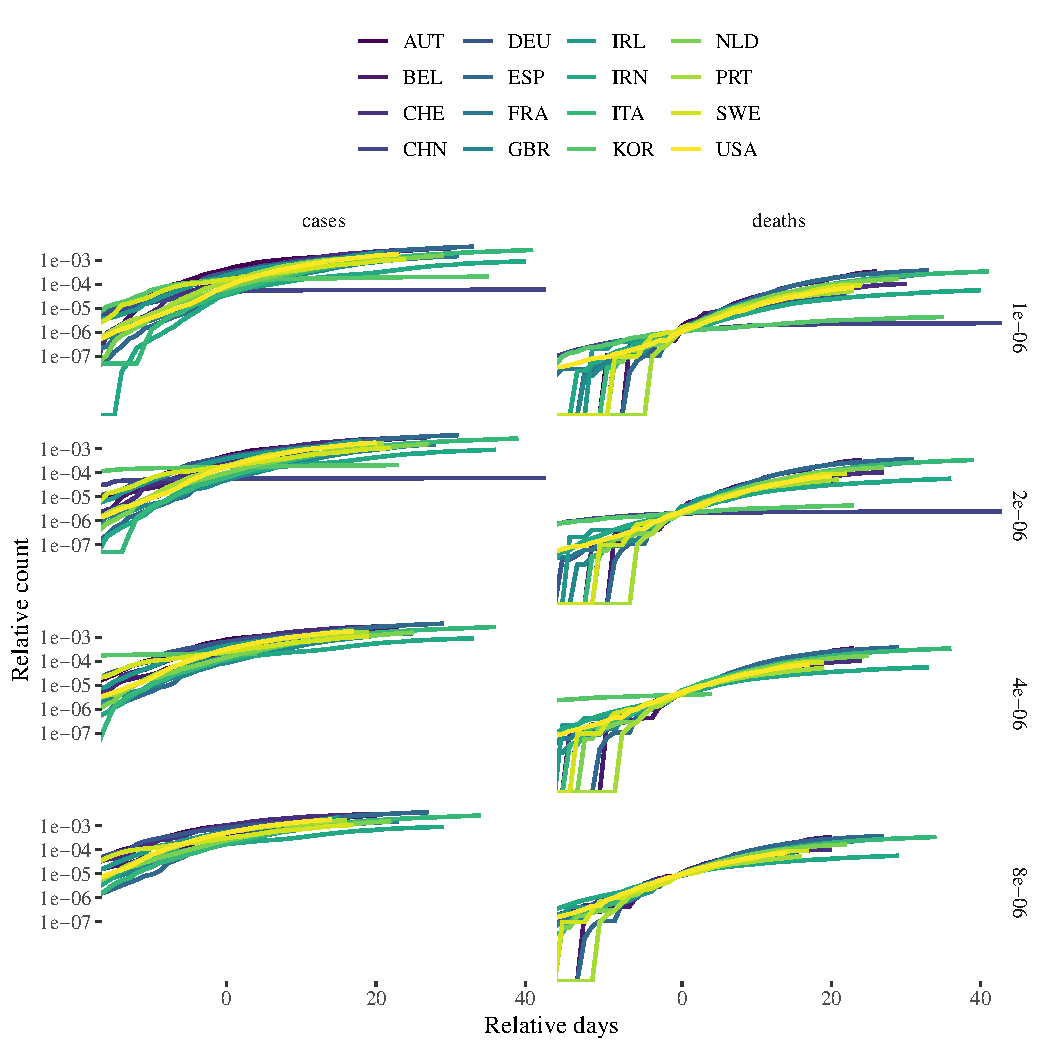
\includegraphics[width=1\textwidth]{../figs/ecdc_align_all.pdf}
  \caption{\label{fig:aligned_data} Relative case and death counts of
    selected countries. Dates are aligned relative to the first day
    that relative death counts exceed one (top) or ten (bottom) per
    million respectively.}
\end{figure}

Here, I do not attempt to explain all these country specific
differences. Instead, the relation between relative death and case
counts is considered. While relative death counts exhibit similar time
courses the corresponding relative case counts $c_t$ are more variable
when aligned in the same fashion, i.e. relative to the first day that
$d_t$ exceeds a given threshold. As I will argue now, most of this
variability can be explained with two readily interpretable
parameters.

\begin{hypothesis}
  \label{hyp:delay}
  There is a well defined country specific delay between reported
  cases and deaths.
\end{hypothesis}

\fig{aligned_data} suggests that relative case counts are not aligned
as some countries, e.g. Germany, systematically lead the counts
reported in other countries, e.g. Italy. Such a difference could mean
that individuals survive longer, e.g. due to differences in medical
care, until they eventually. It could also just reflect reporting
delays due to bureaucratic reasons. In any case, it is clearly the
case that individuals die not immediately, but some days after they
had been tested positive previously.

\subsection{Case fatality rate}

This delay also needs to be taken into account when estimating the
case fatality rate (CFR). Commonly the CFR is defined as $\mathrm{cfr}
= \frac{d_t}{c_t}$. Not surprisingly this estimate is highly variable
and changes systematically over time, especially at the beginning of
an epidemic. The observation captured in \hyp{delay} also explains the
surprisingly low CFRs initially announced in Austria and Germany where
reported death counts are simply some days older compared to other
countries!

Thus, taking into account that individuals that had been tested
positive will usually not die on the same day but after some delay
$\tau$ (if at all), I define
\begin{align}
  \label{eq:cfr}
  \mathrm{cfr}_{\tau} &= \frac{d_t}{c_{t - \tau}} \; ,
\end{align}
i.e. comparing current death with previous case counts.

\begin{figure}
  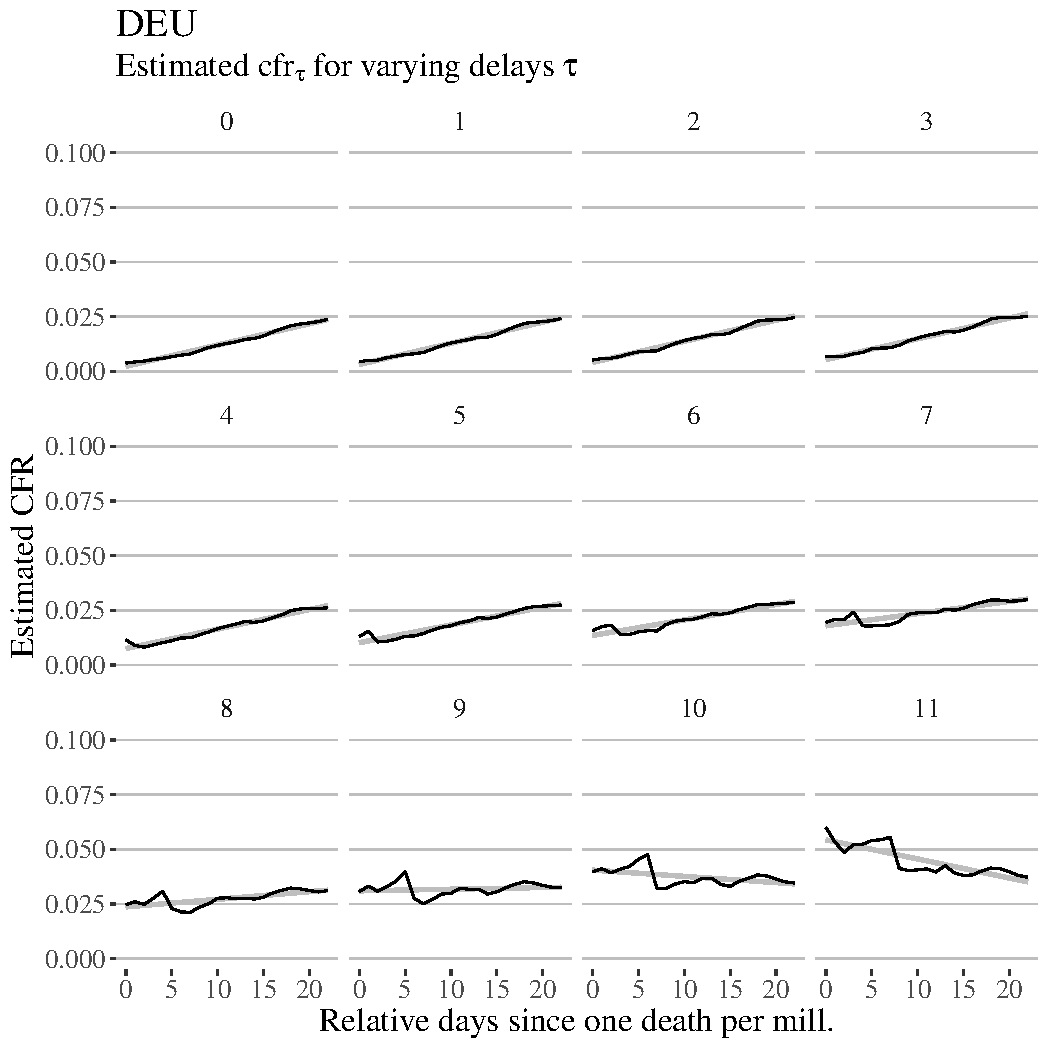
\includegraphics[width=0.495\textwidth]{../figs/ecdc_cfr_delay_DEU.pdf}
  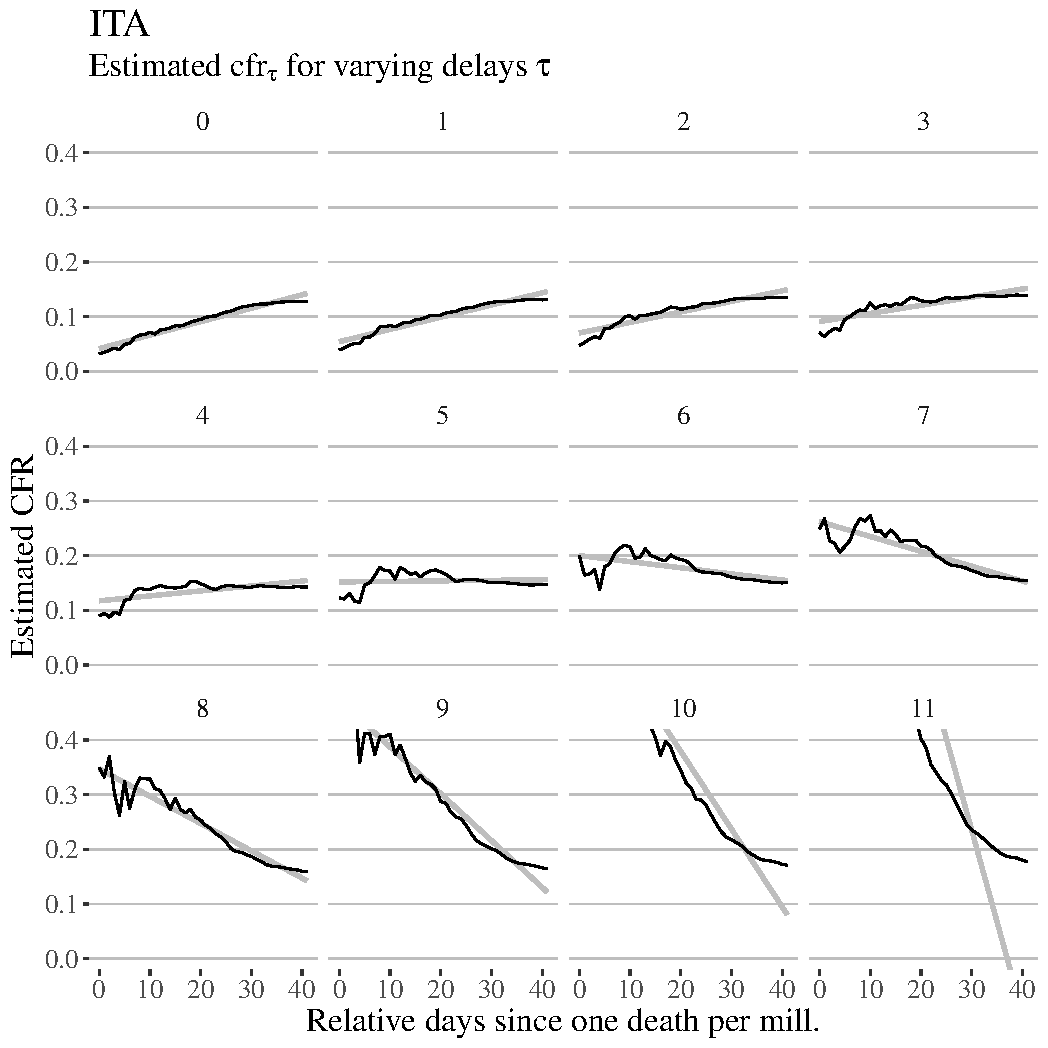
\includegraphics[width=0.495\textwidth]{../figs/ecdc_cfr_delay_ITA.pdf}
  \caption{\label{fig:cfr} Estimated CFR $\mathrm{cfr}_{\tau}$ for
    Germany (left) and Italy (right) using different delays of $\tau =
    0, \ldots, 11$ days. Note that in each case, there exists a
    characteristic delay such that estimates are almost constant over
    time. Further note that estimates for all delays will eventually
    converge to the same final value when enough data are available.}
\end{figure}
\fig{cfr} shows the CFRs estimated for Germany and Italy in this
fashion, i.e. for different delays $\tau$. The estimate using $\tau =
0$ rises over time simply reflecting that due to the reporting delay
death counts have not yet caught up with the exponentially growing
case counts. Interestingly, for each country there exists a
characteristic delay at which the estimated CFRs are essentially
constant. Thus, reflecting the hypothesized delay between reported
cases and deaths.

\begin{hypothesis}
  \label{hyp:cfr}
  The true case fatality rate is the same for all countries.
\end{hypothesis}

\section{Discussion}

In reality, an additional delay between an infection and its
corresponding positive test result can be assumed. Therefore, the
fraction of observed cases will be even lower than obtained by the
analysis above. Unfortunately, assuming a sufficiently flexible model
for the growth of the actual cases already the CFR and the fraction of
observed cases, let alone an additional delay, are not jointly
identifiable.

\subsection{Epidemic modeling}
The basic SIR model \cite{Newman}, assumes that an infection unfolds when
susceptible (S) individuals become infected (I) -- which in turn
infect further susceptible individuals. Finally, infected individuals
recover (R) (or die) and are no longer susceptible. In continuous
time, the dynamics can be described by the following system of
ordinary differential equations (ODEs):
\begin{align*}
  \frac{dS}{dt} &= - \beta \frac{I_t}{N} S_t \\
  \frac{dI}{dt} &= \beta \frac{I_t}{N} S_t - \gamma I_t \\
  \frac{dR}{dt} &= \gamma I_t
\end{align*}
where $N \equiv S_t + I_t + R_t$ is constant over time. Model
parameters are
\begin{itemize}
\item the infection rate $\beta$
\item and the recovery rate $\gamma$.
\end{itemize}
In this model, the average time of infection is $\gamma^{-1}$ giving
rise to a {\em basic reproduction number} of $R_0 = \beta
\gamma^{-1}$.

SIR models and extensions are widely used in epidemic modeling. The
have also been applied to the understand the dynamics of the ongoing
Covid-19 pandemic
\cite{arxiv:2002.07572,arxiv:2004.01105,10.1126/science.abb3221,https://www.medrxiv.org/content/10.1101/2020.02.27.20028639v2}.
In particular, models including the possibility of unobserved cases or
including a reporting delay have been developed. Within the SIR
framework, both effects can be included in several ways, most easily
by assuming that observed cumulative infections are simply a fraction
$\alpha \in [0, 1]$ of previous total infections $I_t + R_t$,
i.e. $\alpha (I_{t - \tau} + R_{t - \tau})$. A more elaborate attempt
instead considers more detailed dynamics of the form
\begin{align*}
  \frac{dS}{dt} &= - \beta_I \frac{S_t}{N} I_t - \beta_O \frac{S_t}{N} O_t - \beta_U \frac{S_t}{N} U_t \\
  \frac{dI}{dt} &= \beta_I \frac{S_t}{N} I_t + \beta_O \frac{S_t}{N} O_t + \beta_U \frac{S_t}{N} U_t - \gamma_I I_t \\
  \frac{dO}{dt} &= \alpha \gamma_I I_t - \gamma_R O_t \\
  \frac{dU}{dt} &= (1 - \alpha) \gamma_I I_t - \gamma_R U_t \\
  \frac{dR}{dt} &= \gamma_R (O_t + U_t)
\end{align*}
where a fraction $\alpha$ of infected individuals $I_t$ is observed
($O_t$) after an initial delay $\frac{1}{\gamma_I}$. In any case,
whether observed or not, individuals recover (or die) after an
additional delay. In general, the infection rates $\beta_I, \beta_O,
\beta_U$ could be different for initial infections and observed vs
unobserved cases\footnote{An effective quarantine would be modeled via
  $\beta_O \equiv 0$.}.

In addition, mitigation measures, e.g. social distancing, can be
easily included by assuming that $\beta$'s are functions of
time. E.g. \cite{arxiv:2004.01105} assumes one or several (soft) step
functions where $\beta$ drops after measures have been
implemented. Unfortunately, as we show now a model including a
time-varying $\beta$ as well as unobserved cases is not identifiable.
For simplicity, consider the above model with $\beta_I = \beta_O =
\beta_U =: \beta$. Then, new infections arise with intensity $\beta
\frac{S_t}{N} (I_t + O_t + U_t)$ which in turn translate into observed
cases with intensity $\alpha \gamma_I I_t$. Now assume a second model
with $\alpha' = 1 > \alpha$. By using a time varying $\beta'(t)$
such that
\begin{align*}
  \beta'(t) &= \alpha \beta \frac{S_t}{S'_t}
\end{align*}
we obtain exactly the same number of observed cases $O_t$. Note that
as $\alpha' > \alpha$, we have that $S_t < S'_t$ and $S_t$ is a
sigmoidal function of time due to the SIR dynamics. Furthermore, when
the population is large, i.e. $N \gg 1$ and $S_0 \approx N$ the
resulting $\beta'(t)$ is mostly driven by the drop in $S_t$ as
compared to the much smaller change in $S'_t$. Indeed, \fig{SIRapprox}
shows the dynamics of the above model with $\beta = 0.3, \gamma_I =
\gamma_R = \frac{2}{10}$\footnote{Giving rise to an $R_0$ of $3$.} and
$\alpha = 0.1$ starting from $(N = 10^8, 1, 0, 0, 0)$. In turn, the
dynamics is approximated by the best-fitting logistic sigmoid scaling
$\beta'(t)$ and assuming $\alpha' = 1$. Note that the number of
observed cases is almost identical whereas the final fraction of
susceptible individuals is vastly different. Indeed, in the first case
the epidemic is stopped by group immunity whereas in the second case
effective mitigation measures are imposed. Correspondingly, police
implications would be vastly different in the two situations even
though they are observationally indistinguishable.
\begin{figure}
  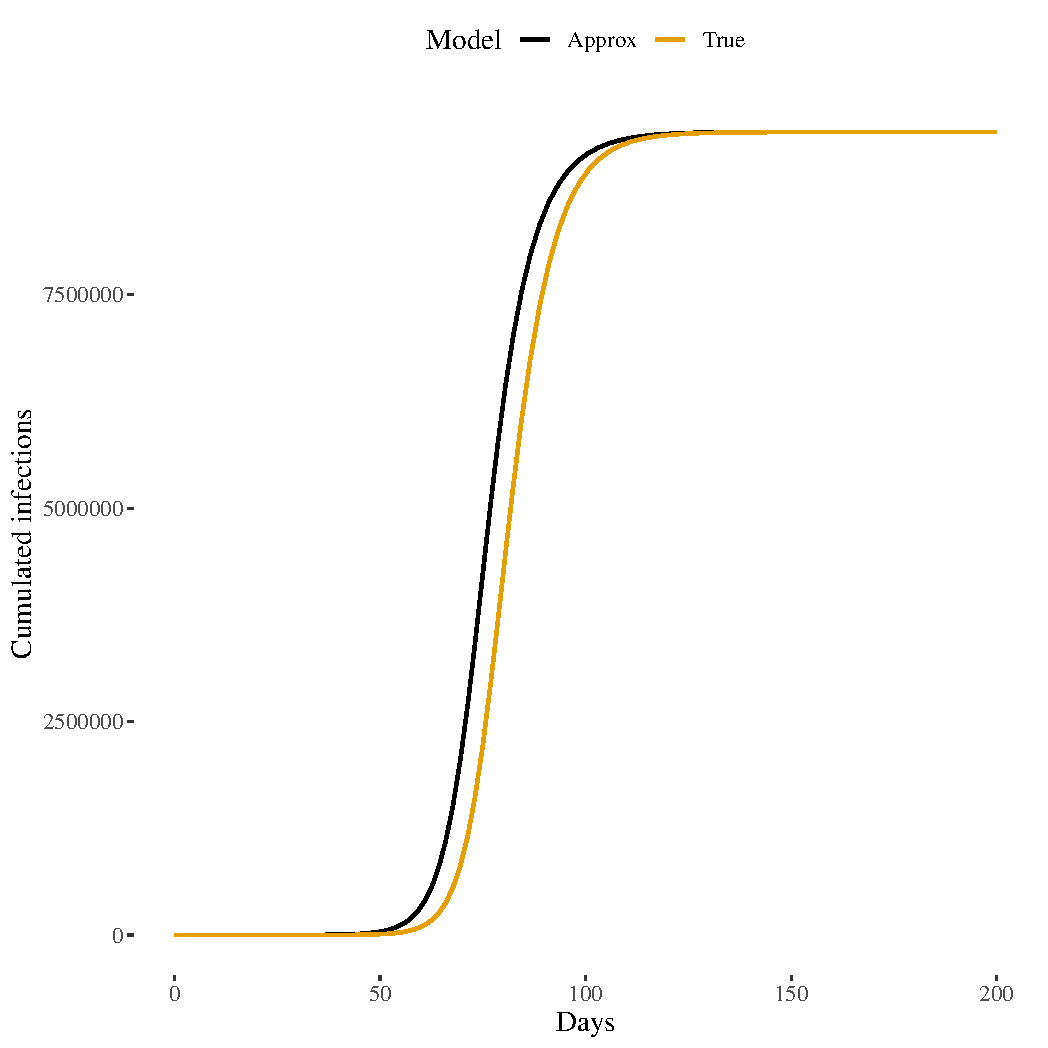
\includegraphics[width=0.45\textwidth]{../figs/approx_infect.pdf}
  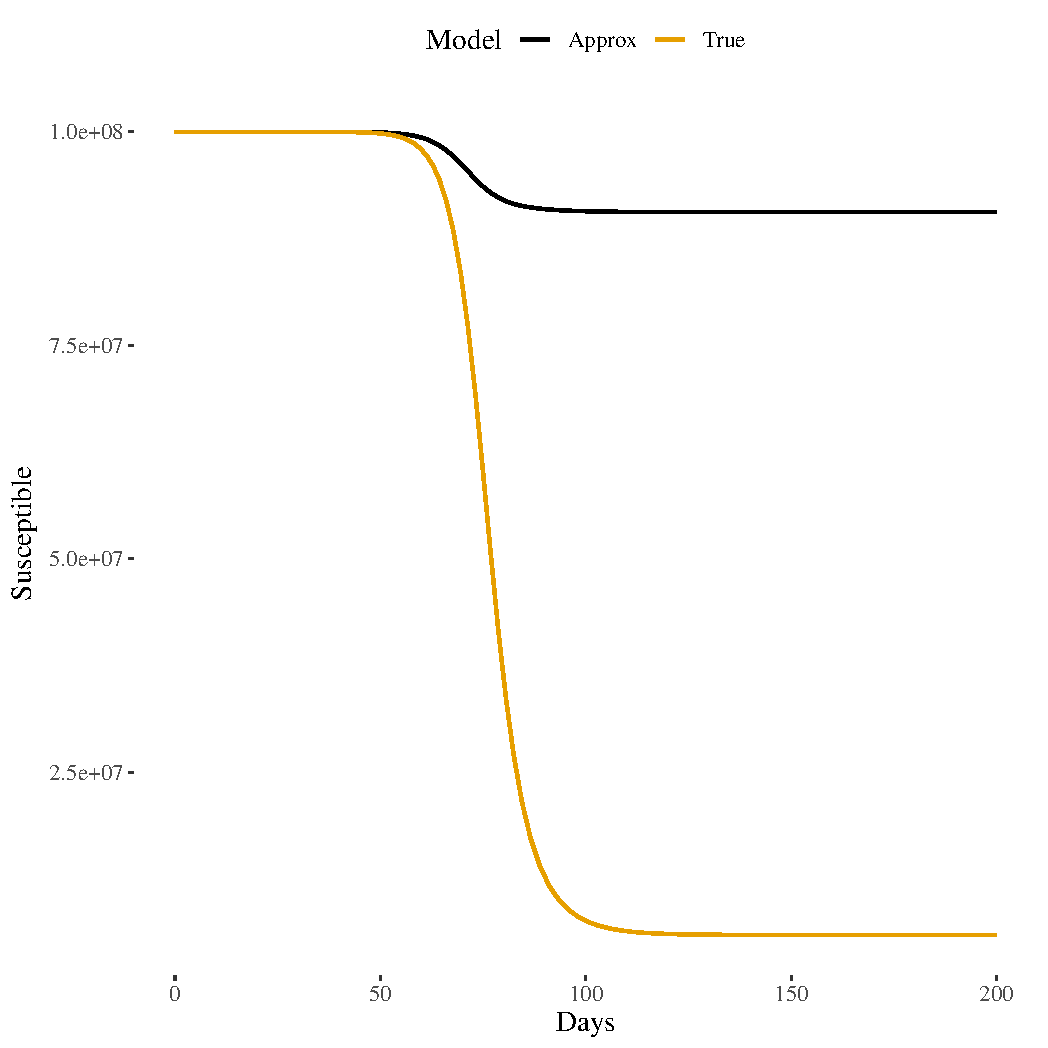
\includegraphics[width=0.45\textwidth]{../figs/approx_suscept.pdf}
  \caption{\label{fig:SIRapprox} Total cumulative observed infections
    and number of susceptible individuals in two simulated model with
    observation fraction $\alpha = 0.1$ (true) and observation
    fraction $\alpha' = 1$ (approx). In the second model, the epidemic
    is stopped due to mitigation measures which are modeled via
    $\beta'(t)$ as explained in the main text.}
\end{figure}

\subsection{Implications}

Furthermore, containment is challenging due to week
long incubation times
\cite{https://doi.org/10.1101/2020.03.25.20043109} but a conbination
of case tracing and isolation policies could be effective
\cite{fraser04,kubinec}. On the other hand, if most cases are actually
known effective policies can be implemented as evidenced in the
currently successful containment in China and South Korea. In the end,
data analysis alone only gets us only that far and more extensive
testing is urgently needed.


\bibliographystyle{abbrv}
\bibliography{notes}

\clearpage

\appendix
\renewcommand\appendixname{Supplement}
\beginsupplement

\section{Additional figures}

\begin{figure}
  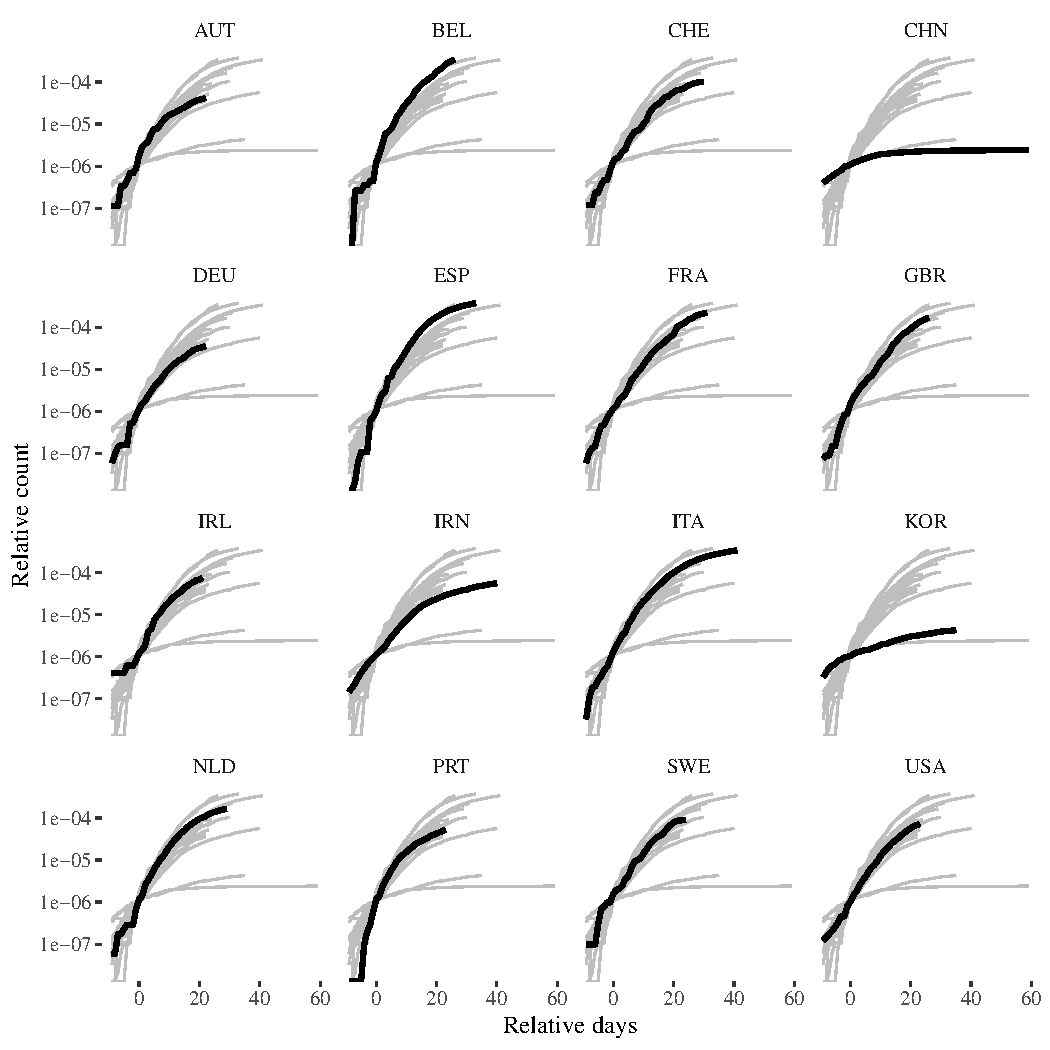
\includegraphics[width=1\textwidth]{../figs/ecdc_aligned_onepermill_nyt.pdf}
  \caption{\label{fig:align_nyt}}
\end{figure}

\section{Uncertainty estimates from SIR model}

Note that an SIR model already includes a natural delay between
infections and recovery (or death). Indeed, the total number of cases
is given by $C_t = I_t + R_t$ while the cumulated death toll is
obtained as $\mathrm{cfr} R_t$, i.e. modeling that a fraction of
individuals does not recover but dies instead. Assuming that only a
fraction $\alpha$ of cases is observed, the model is estimated with
the following sampling distribution
\begin{align*}
  C^{\mathrm{obs}}_{t+1} - C^{\mathrm{obs}}_t &\sim \mathrm{NegativeBinomial}\left(\alpha \frac{dC^{\mathrm{model}}_t}{dt}, \phi_C \right) \\
  D^{\mathrm{obs}}_{t+1} - D^{\mathrm{obs}}_t &\sim \mathrm{NegativeBinomial}\left(\mathrm{cfr} \frac{dR^{\mathrm{model}}_t}{dt}, \phi_D \right) \; .
\end{align*}
Thus, observed daily changes are related to the model implement
changes via an overdispersed Poisson aka negative binomial
distribution. \fig{sir_fit} shows the resulting estimates assuming
$\beta_t = \beta_1 + (\beta_2 - \beta_1) \frac{1}{1 + e^{- \frac{t -
      \tau}{T} }}$ and $\mathrm{cfr} = 1\%$\footnote{Due to the
  non-identifiability derived in the main text either $\alpha$ or
  $\mathrm{cfr}$ needs to be fixed.}.

\begin{figure}
  
  \caption{\label{fig:sir_fit}}
  
\end{figure}

\end{document}
